%======================================================================
% L5a_Potentials.pdf
%======================================================================
\providecommand{\tg}{\operatorname{tg}}
% přeškrtnutí v rovnici (balík cancel není k dispozici)
\providecommand{\cancel}[1]{\tikz[baseline=(c.base)]{\node[inner sep=0pt](c){$#1$};\draw[NavyBlue](c.south west)--(c.north east);}}
\section{Termodynamické potenciály}
\strana{L5a-1}

\begin{itemize}
  \item $U(S,X,\xi)$ je fund.\ rovnice splňující princip extrému $[\delta U]_{S,X}\geq 0$
  \item pro $U(T,X,\xi)$ nebo $U(S,y,\xi)$ už ale nic takového neplatí, navíc $\left(\pdv{U}{X}\right)_{T,\xi}\neq y$ $\Rightarrow$ $U(T,X,\xi)$ neobsahuje info o stav.\ rovnicích
\end{itemize}
\noindent\rule{\linewidth}{0.4pt}

\subsection{Legendreova transformace}
\begin{itemize}
  \item uvažujme funkci $y = y(x)$ \ \& \ $p \equiv \dfrac{\dd y}{\dd x}$
\end{itemize}
\underline{Otázka:} jak zkonstruovat funkci $y = y(p)$ bez ztráty informace?

\begin{priklad}[Př:]
\begin{itemize}
  \item $y = \frac{1}{10}x^2 \ \Rightarrow\ p = \frac15x \ \Rightarrow\ y(p) = \frac52p^2$
  \item jak se dostanu zpět k $y = y(x)$, znám-li pouze $y(p)$ a $p = \dfrac{\dd y}{\dd x}$?
\end{itemize}
$\to$ mám vlastně rovnici \quad $y(x) = \dfrac52\left(\dfrac{\dd y}{\dd x}\right)^2$
\[
  \to\ \dd x = \sqrt{\tfrac52}\,\frac{\dd y}{y^{1/2}}
  \ \Rightarrow\ \sqrt{\tfrac25}\,x = 2\sqrt y - 2C
  \ \Rightarrow\ y = \Big(x\sqrt{\tfrac{1}{10}} + C\Big)^2
\]
\[
  \Rightarrow\ y = \frac1{10}x^2 + 2Cx\sqrt{\tfrac1{10}} + C^2 = \frac{1}{10}(x + x_0)^2
\]

\begin{minipage}{0.45\textwidth}
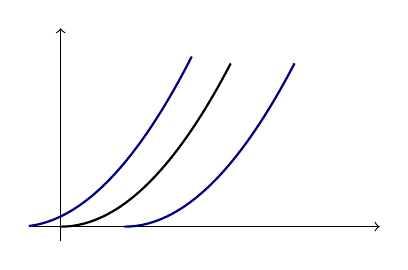
\begin{tikzpicture}[scale=0.9]
  \draw[->] (-0.4,0) -- (4.5,0);
  \draw[->] (0,-0.2) -- (0,2.8);
  \draw[thick,domain=0:2.4,samples=40] plot (\x,{0.4*\x*\x});
  \draw[NavyBlue,thick,domain=-0.45:1.85,samples=40] plot (\x,{0.4*(\x+0.6)*(\x+0.6)});
  \draw[NavyBlue,thick,domain=0.9:3.3,samples=40] plot (\x,{0.4*(\x-0.9)*(\x-0.9)});
\end{tikzpicture}
\end{minipage}
\begin{minipage}{0.5\textwidth}
$\leftarrow$ tento naivní postup mám po transformaci zpět dává libovolně posunutou parabolu
\end{minipage}
\end{priklad}

%----------------------------------------------------------------------
\strana{L5a-2}
\begin{itemize}
  \item jednoznačné určení původní funkce získáme tehdy, pokud vedle derivace $p = \frac{\dd y}{\dd x}$ (směrnice tečny) budeme znát také průsečík tečny s osou $\langle y\rangle$ $\Leftrightarrow$ funkci $y(x)$ popíšeme obálkou jejích tečen
\end{itemize}

\begin{minipage}{0.6\textwidth}
\begin{tikzpicture}[scale=0.85,>=Stealth]
  \draw[->] (-0.5,0) -- (7.5,0) node[below] {$x$};
  \draw[->] (0,-0.5) -- (0,5.4) node[left] {$y$};
  % funkce
  \draw[thick] (-0.05,1.6) .. controls (1,1.6) and (2,2) .. (3,2.65)
               .. controls (3.6,3.1) and (4.1,3.6) .. (4.6,4.3) node[above] {$y(x)$};
  % tečna (červená)
  \draw[Red,thick] (-0.2,1.0) -- (6.1,4.5);
  \draw[Red] (0.5,1.4) arc (30:5:0.6);
  \node[Red,rotate=30] at (1.5,1.8) {$\tg\alpha = p$};
  % rovnoběžky (modré)
  \draw[NavyBlue,thick] (-0.4,1.8) -- (5.6,5.3);
  \draw[NavyBlue,thick] (-0.25,0.2) -- (5.9,3.8);
  \node[NavyBlue] at (5.3,5.15) {$\times$};
  \node[NavyBlue] at (5.6,3.6) {$\times$};
  % pomocné čáry
  \draw[OliveGreen,dotted] (0,2.65) -- (3,2.65) -- (3,0);
  \draw[Red,dotted] (0,1.08) -- (7,1.08);
  \node[left] at (0,2.65) {$Y$};
  \node[left,Red] at (0,1.08) {$\psi$};
  \node[below] at (3,0) {$X$};
\end{tikzpicture}
\end{minipage}
\begin{minipage}{0.38\textwidth}
\begin{itemize}
  \item $\tg\alpha = p = \dfrac{Y - \psi}{X - 0}$
\end{itemize}
\[ \Rightarrow\ Y - \psi = pX \]
\[ \Rightarrow\ \psi = Y - pX \]
\end{minipage}

\begin{definice}[Legendreova transformace]
$\Rightarrow$ \kw{Legendreova transformace} fce $y = y(x)$ s $\dfrac{\dd y}{\dd x}\equiv p$ je funkce
\[
  \vzorec{\psi(p) = y(p) - p\,x(p)}
\]
\end{definice}
\begin{itemize}
  \item inverzní Leg.\ transformace:
  \[
    \dd\psi = \underbrace{\dd y - p\,\dd x}_{\equiv 0 \text{ z def.\ } p} - x\,\dd p = -x\,\dd p
    \quad\Rightarrow\quad x = -\frac{\dd\psi}{\dd p}
  \]
\end{itemize}
\begin{center}$\Downarrow$\end{center}
\begin{center}
\begin{tabular}{|p{0.42\textwidth}|p{0.42\textwidth}|}
\hline
\textbf{LT:} & \textbf{ILT:} \\
$y = y(x)$ & $\psi = \psi(p)$ \\
$p \equiv \dfrac{\dd y}{\dd x}\ \Rightarrow\ x = x(p)$ \ \textcolor{NavyBlue}{\small $\leftarrow$ invertuji} &
$x = -\dfrac{\dd\psi}{\dd p}\ \Rightarrow\ p = p(x)$ \\[8pt]
$\psi(p) = y(p) - p\,x(p)$ & $y(x) = \psi(x) + x\,p(x)$ \\
\hline
\end{tabular}
\end{center}

%----------------------------------------------------------------------
\strana{L5a-3}
\begin{itemize}
  \item operace je symetrická: v obou případech
  \[ F(z) = f - \left(\pdv{f}{x}\right)x = f - z\,x(z) \]
\end{itemize}

\begin{priklad}[Př:]
\begin{itemize}
  \item $y = \frac1{10}x^2 \Rightarrow p = \frac15x \Rightarrow x = 5p \Rightarrow \psi(p) = \frac52p^2 - 5p^2$
  \[ \Rightarrow\ \psi(p) = -\frac52p^2 \]
  \item $x = -\dfrac{\dd\psi}{\dd p} = 5p \Rightarrow p = \frac15x \Rightarrow y(x) = -\frac52\left(\frac{x}{5}\right)^2 + \frac15x^2$
  \[ \Rightarrow\ y(x) = -\frac1{10}x^2 + \frac{2}{10}x^2 = \frac1{10}x^2 \quad\checkmark \]
\end{itemize}
\end{priklad}
\begin{center}\rule{0.6\linewidth}{0.4pt}\end{center}

\begin{veta}[Fundamentální rovnice v intenzivních veličinách]
$\Rightarrow$ fundamentální rovnice v reprezentaci vybraných intenzivních veličin dostaneme prostřednictvím Legendreových transformací $y_i\leftrightarrow X_i$
\end{veta}
\begin{itemize}
  \item z konstrukce vyplývá, že umíme zaměňovat pouze \underline{sdružené proměnné} \quad $y_i = \left(\pdv{U}{X_i}\right)\leftrightarrow X_i$
\end{itemize}

\begin{minipage}{0.68\textwidth}
\begin{itemize}
  \item obecně: \ $Y = Y(X_1,\dots,X_n) \leftrightarrow \dd Y = \sum y_i\dd X_i$
  \[
    \Rightarrow\ \psi = \psi(y_1,\dots,y_r,X_{r+1},\dots,X_k) = Y - \sum_{i=1}^{r}y_iX_i
  \]
  \[
    \Rightarrow\ \vzorec{\dd\psi = -\sum_{i=1}^{r}X_i\,\dd y_i + \sum_{j=r+1}^{k}y_j\,\dd X_j}
  \]
\end{itemize}
\end{minipage}\hfill
\begin{minipage}{0.3\textwidth}
\fbox{\parbox{\linewidth}{\underline{Pozorování:} \\
$y$ konvexní v $x$ \\
\hspace*{1.2cm}$\Updownarrow$ \\
$\psi$ konkávní v $p$ \\[3pt]
$\dfrac{\dd^2y}{\dd x^2} = \dfrac{\dd p}{\dd x} > 0$ \\[3pt]
$\Rightarrow \dfrac{\dd^2\psi}{\dd p^2} = -\dfrac{\dd x}{\dd p} < 0$}}
\end{minipage}

\begin{itemize}
  \item známe Lagrange $\to$ Hamilton:
  \[
    \mathcal{L} = \mathcal{L}(\dot q_i, q_i) \ \to\ \mathcal{H} = \mathcal{H}(p_i,q_i) = \sum_i p_i\dot q_i - \mathcal{L}
    \qquad p_i = \pdv{\mathcal{L}}{\dot q_i}
  \]
\end{itemize}

%----------------------------------------------------------------------
\strana{L5a-4}
\subsection{Helmholtzova volná energie}
\begin{itemize}
  \item složený systém se skládá z podsystému $\mathcal{S}$ a lázně $\mathcal{L}$; \ $|\mathcal{L}|\gg|\mathcal{S}| \Leftrightarrow C^{\mathcal{L}}\gg C$
  \quad \textcolor{NavyBlue}{\small (lázeň: $C^{\mathcal{L}}\to\infty$)} \\
  \textcolor{NavyBlue}{\small \hfill veličiny příslušné k $\mathcal{S}$ neindexuji}
  \begin{enumerate}[label=\roman*)]
    \item bez ohledu na tepelnou výměnu lze teplotu lázně považovat za konstantní
    \item víme, že v rovnováze bude teplota $\mathcal{S}$ rovna teplotě lázně
  \end{enumerate}
  $\Rightarrow$ lázeň pouze zprostředkovává konstantní teplotu; místo vnitřní energie celého složeného systému bychom chtěli pracovat s nějakou veličinou dimenze energie, která by se vztahovala pouze k $\mathcal{S}$ a byla funkcí $T$ a $X_i$
  \item chceme, aby tato veličina splňovala princip extrému (minima) vůči $X_i$ (hodnotu $T$ známe) a navíc \uv{obsahovala} i stavové rovnice
  \item uvažujme tedy kompozitní systém popsaný fund.\ rovnicí \textcolor{NavyBlue}{\small $\overset{?}{=}U^t(S^t,X;\xi,S)$}
  \[
    U^t = U^t(S,X,\xi;S^{\mathcal{L}}) = U(S,X,\xi) + U^{\mathcal{L}}(\underbrace{S^{\mathcal{L}}}_{\textcolor{NavyBlue}{S^t - S}})
  \]
  $\to$ rovnováha: \ $\dd U^t = 0$ \ \& \ $\dd^2U^t > 0$
  \begin{itemize}[nosep]
    \item navíc platí $\dd S^t = \dd(S + S^{\mathcal{L}}) = 0$ \hfill \textcolor{NavyBlue}{\small $S^t = S^{\mathcal{L}} + S$} \\
    $\Leftarrow$ princip minima $U^t$ předp.\ konst.\ entropii \\
    $\Leftarrow$ v rovnováze $T = T^{\mathcal{L}}$ \& $\dd Q = -\dd Q^{\mathcal{L}} \Rightarrow \dd S = -\dd S^{\mathcal{L}}$
  \end{itemize}
\end{itemize}
\begin{align*}
  a)\quad \dd U^t &= \dd U + \dd U^{\mathcal{L}} = \big/\,\dd U^{\mathcal{L}} = \dd Q^{\mathcal{L}}\,\big/ = \dd U + T^{\mathcal{L}}\dd S^{\mathcal{L}} \\
  &= \big/\,\dd S^{\mathcal{L}} = -\dd S\,\big/ = \dd U - T^{\mathcal{L}}\dd S
\end{align*}

%----------------------------------------------------------------------
\strana{L5a-5}
\begin{itemize}
  \item přitom $T = T^{\mathcal{L}} = \text{konst}$
  \[ \Rightarrow\ \boxed{\dd U^t = \dd(U - TS) = \dd F} \]
  \item definuji \underline{Helmholtzovu volnou energii}
\end{itemize}
\begin{definice}[Helmholtzova volná energie]
\[
  \vzorec{F(T,X,\xi) = U - TS} \qquad \big/\,S = S(T,X,\xi)
\]
\end{definice}
\begin{itemize}[nosep]
  \item[$\to$] je to přirozeně funkce $T,X,\xi$, neboť $T$ je zde kontrolovaný parametr, nikoliv $S$
  \item[$\to$] navíc $F = F(T,X,\xi)$ je Leg.\ transformací $U = U(S,X,\xi)$ $\Rightarrow$ je to \uv{bezztrátová} transformace
  \item[$\to$] $F$ se vztahuje pouze k $\mathcal{S}$, $U^{\mathcal{L}}(S^{\mathcal{L}})$ se v def.\ nevyskytuje; $\mathcal{L}$ je \uv{přítomna implicitně} skrze kontrolovanou $T$
  \item[$\to$] v rovnováze $[\dd F]_{T,X} = 0$, neboť $[\dd U^t]_{T,X} = [\dd F]_{T,X}$
\end{itemize}
\begin{itemize}
  \item Nabývá $F$ extrému? Jakého typu? \hfill \textcolor{NavyBlue}{($\ast$ viz dále)}
\end{itemize}
\begin{align*}
  \dd^2(U - TS)\big/_T &= \big/\,U = U(S,X;\xi)\,\big/ \\
  &= \frac{\partial^2}{\partial S^2}(U - TS)(\dd S)^2 + \sum_i\frac{\partial^2}{\partial\zeta_i\partial S}(U - TS)\,\dd S\,\dd\zeta_i \\
  &\quad + \sum_{i,j}\frac{\partial^2}{\partial\zeta_i\partial\zeta_j}(U - TS)\,\dd\zeta_i\,\dd\zeta_j
   = \big/\,S, \zeta_i \text{ nezávislé},\ T = \text{konst}\,\big/ \\
  &= \frac{\partial^2U}{\partial S^2}(\dd S)^2 + \sum_i\frac{\partial^2U}{\partial\zeta_i\partial S}\dd S\,\dd\zeta_i + \sum_{ij}\frac{\partial^2U}{\partial\zeta_i\partial\zeta_j}\dd\zeta_i\,\dd\zeta_j \\
  &= \dd^2U \qquad\Rightarrow\quad \textcolor{NavyBlue}{\boxed{\dd^2F = \dd^2U}}
\end{align*}
\begin{itemize}
  \item my ovšem víme $\dd^2U^t = \dd^2U + \dd^2U^{\mathcal{L}} > 0$
\end{itemize}

%----------------------------------------------------------------------
\strana{L5a-6}
$\to$ platí $|\dd^2U^{\mathcal{L}}|\ll\dd^2U$:
\[
  \dd^2U^{\mathcal{L}} = \left(\frac{\partial^2U^{\mathcal{L}}}{\partial(S^{\mathcal{L}})^2}\right)(\dd S^{\mathcal{L}})^2
  \underset{\dd S^{\mathcal{L}} = -\dd S}{=}
  \underbrace{\left(\frac{\partial^2U^{\mathcal{L}}}{\partial(S^{\mathcal{L}})^2}\right)}_{\textcolor{NavyBlue}{\propto\frac{1}{N^{\mathcal{L}}}}}
  \underbrace{(\dd S)^2}_{\textcolor{NavyBlue}{\propto N^2}}
  \propto \frac{N^2}{N^{\mathcal{L}}} \xrightarrow{\ N^{\mathcal{L}}\to\infty\ } 0
\]
\[
  \dd^2U\propto N \qquad\qquad \Rightarrow\quad \boxed{\frac{\dd^2U^{\mathcal{L}}}{\dd^2U}\propto\frac{N}{N^{\mathcal{L}}}\to 0}
\]
\[
  \Rightarrow\quad \textcolor{NavyBlue}{\boxed{\dd^2U^t > 0 \Leftrightarrow \dd^2U > 0 \Leftrightarrow \dd^2F > 0}}
  \quad \pozn{v originále omylem psáno \uv{$= 0$}}
\]
$\Rightarrow$ dostáváme podmínku rovnováhy
\[
  \textcolor{NavyBlue}{\boxed{[\delta F]_{T,X}\geq 0}} \qquad \textcolor{NavyBlue}{\text{princip minima pro H.\ volnou energii}}
\]
$\Rightarrow$ $F = F(T,X;\xi)$ je plnohodnotná fundament.\ rovnice

\begin{veta}[Princip minima Helmholtzovy volné energie]
\textcolor{Red}{Rovnovážné hodnoty volných vnitřních extenzivních veličin v systému v tepelném kontaktu s lázní minimalizují Helmholtzovu volnou energii na \underline{podprostoru stavů s teplotou $T = T^{\mathcal{L}}$}.}
\end{veta}
\begin{itemize}
  \item \pozor{$F$ konvexní v $X,\xi$, konkávní v $T$!}
  \item \underline{diferenciál a Eulerova rovnice:}
  \[
    \vzorec{\dd F = -S\,\dd T + \sum y_i\,\dd X_i}
  \]
  \[
    F = U - TS = \sum y_iX_i \underset{\text{\small jednoduchý syst.}}{=} -pV + \mu N
  \]
  \item \underline{fyzikální význam:}
  \[
    [\Delta F]_T = W \quad\dots\ \text{práce dostupná v izotermickém procesu}
  \]
\end{itemize}

%----------------------------------------------------------------------
\strana{L5a-7}
\begin{itemize}
  \item obvyklé značení: \quad $F(T,X) = U[T](T,X)$
  \item vnitřní energie $U(T,X)$ z $F(T,X)$:
  \[
    U = F + TS = F - T\left(\pdv{F}{T}\right)_X = -T^2\left(\frac{\partial(F/T)}{\partial T}\right)_X
  \]
  \textcolor{NavyBlue}{\underline{NB:} \ $-\dfrac{F}{T} = S\big[\tfrac1T\big](T,X)$}
\end{itemize}

\underline{NB:} $\bullet$ Clausius: \ $T\dd S\geq\dd U - \dd W$
\[
  \dd F = \dd U - T\dd S - S\dd T \ \Rightarrow\ \dd U = \dd F + T\dd S + S\dd T
\]
\[
  \Rightarrow\ 0\geq\dd F + S\dd T - \dd W \ \Rightarrow\ \big/\,\dd W = \dd T = 0\,\big/ \ \Rightarrow\ \dd F\leq 0
\]
$\Rightarrow$ v nevratném procesu $[\dd F]_{T,X}\leq 0$ \\
$\Rightarrow$ směrem do rovnováhy $F$ klesá, v rovnováze $[\delta F]_{T,X} > 0$ \dots\ $F$ je minimální

\begin{itemize}
  \item $F = U - TS$ v sobě obsahuje oba základní fyzikální principy: $U$ směřuje do minima a $S$ do maxima -- obě tendence $S\nearrow$ a $U\searrow$ vedou k $F\searrow$
  \item entropický a energetický princip by ale samostatně vedly k jiným rovnováhám;
  \[
    \min F\ \begin{array}{l}\sim\ \max S \\ \times \\ \sim\ \min U\end{array}
  \]
  ($S$ a $U$ nejsou nezávislé $\Rightarrow$ nelze za konst.\ $T$ zároveň $\max S$ a $\min U$)
\end{itemize}

%----------------------------------------------------------------------
\strana{L5a-8}
\textcolor{NavyBlue}{
\begin{itemize}
  \item zkusme to ještě alternativně: ($\ast$)
\end{itemize}
\begin{align*}
  \dd^2F\big|_{T,X} &= \dd^2\Big[U\big(S(T,X;\xi),X;\xi\big) - T\,S(T,X;\xi)\Big] \\
  &= \frac{\partial^2U}{\partial\xi_i\partial\xi_j}\dd\xi_i\dd\xi_j - \underset{T = \text{konst}}{T}\left(\frac{\partial^2S}{\partial\xi_i\partial\xi_j}\right)\dd\xi_i\dd\xi_j \\
  &= \pdv{\xi_i}\left[\left(\pdv{U}{S}\right)_{X,\xi}\left(\pdv{S}{\xi_j}\right)_T + \left(\pdv{U}{\xi_j}\right)_{S,X}\right]\dd\xi_i\dd\xi_j
     - T\left(\frac{\partial^2S}{\partial\xi_i\partial\xi_j}\right)\dd\xi_i\dd\xi_j \\
  &= T\left(\frac{\partial^2S}{\partial\xi_i\partial\xi_j}\right)\dd\xi_i\dd\xi_j + \left(\frac{\partial^2U}{\partial\xi_i\partial\xi_j}\right)\dd\cdot\dd \\
  &\quad - \ \ /\!/\ \ -
\end{align*}
$\Rightarrow$ indeed, $[\dd^2F]_{T,X} = [\dd^2U]_{T,X}$ \ \checkmark \\
toto je zřejmě čistší odvození\dots}

%----------------------------------------------------------------------
\strana{L5a-9}
\begin{itemize}
  \item zobecnění postupu na další páry sdružených prom.
  \item v dalším budeme spec.\ uvažovat systém charakterizovaný $S, V, N_1,\dots,N_l$ \\
  $\to$ tedy fund.\ rovnicí $U(S,V,N_1,\dots)$ nebo $F(T,V,N_1,\dots)$
\end{itemize}

\subsection{Entalpie \quad $H(S,p,N_1,\dots) = U[p]$}
\begin{definice}[Entalpie]
\[
  \vzorec{H = U(S,p,N_1,\dots) + pV(S,p,N_1,\dots)} \ \underset{\text{Euler (ext.)}}{=}\ TS + \sum_i\mu_iN_i
\]
\end{definice}
\begin{itemize}
  \item $\dd H = \dd U + \dd(pV) = \dd U + p\dd V + V\dd p$ \quad $\Rightarrow$
\end{itemize}
\[
  \boxed{\dd H = T\dd S\ \textcolor{Red}{\underline{\textcolor{black}{+V\dd p}}} + \sum\mu_i\dd N_i}
  \qquad
  \textcolor{NavyBlue}{\small\begin{array}{l}
    \text{zobecnění:} \to \\
    \dd U = T\dd S + \vec y\cdot\dd\vec X + \sum\mu_j\dd N_j \\
    \Rightarrow \dd H = T\dd S - \vec X\cdot\dd\vec y + \sum\mu_j\dd N_j
  \end{array}}
\]
\[
  T\equiv\left(\pdv{H}{S}\right)_{p,N_i}\qquad V\equiv\left(\pdv{H}{p}\right)_{S,N_i}\qquad \mu_i\equiv\left(\pdv{H}{N_i}\right)_{S,p,N_{j\neq i}}
\]
$\to$ $\forall$ jako funkce přirozených proměnných $H$

\begin{itemize}
  \item \underline{princip minima:} \hfill \textcolor{Red}{$\dd W'$: $\dd W + p\dd V$ \dots\ jiná než mech.\ práce}
  \[
    T\dd S\geq\dd Q = \dd(U + pV) - V\dd p - \sum\mu_i\dd N_i
  \]
  \[
    \Rightarrow\ \dd H\leq T\dd S + V\dd p + \dd W'
  \]
  \[
    \begin{array}{c}\dd p = 0\\ \Rightarrow\\ \dd N_i = 0\end{array}
    \quad \dd H\leq T\dd S \ \Leftrightarrow\
    \boxed{[\Delta S]_{H,p,N_i}\geq 0 \ \ \&\ \ [\Delta H]_{S,p,N_i}\leq 0}
  \]
  \[
    \Rightarrow\ \vzorec{[\delta H]_{S,p,N}\geq 0}
  \]
  $\Rightarrow$ entalpie nabývá minima na podprostoru stavů $p = p_0$ (tj.\ popisuje systém v kontaktu s \uv{mechanickým rezervoárem})
  \item \underline{fyzikální význam:} \quad $\dd Q = \dd H - V\dd p - \sum\mu_i\dd N_i$
  \[
    \vzorec{[\Delta H]_{p,N_i} = \dd Q \ \Rightarrow\ C_p = \left(\frac{\dd H}{\dd T}\right)_{p,N_i}}
    \qquad
    \textcolor{NavyBlue}{\small\begin{array}{l}\text{srov.}\\ \dd Q = \dd U + p\dd V - \sum\mu_j\dd N_j\\ \Rightarrow C_V = \left(\pdv{U}{T}\right)_{V,N_i}\end{array}}
  \]
  \item také $[\Delta H]_{S,p} = (\dd W')_{\text{ad}}$
\end{itemize}

%----------------------------------------------------------------------
\strana{L5a-10}
\subsection{Gibbsův potenciál \quad $G(T,p,N_1,\dots) = U[T,p]$}
\begin{definice}[Gibbsův potenciál]
\[
  \begin{aligned}
    &\vzorec{G(T,p,N_1,\dots) = U(T,p,N_1,\dots) + pV(T,p,\dots) - TS(T,p,\dots)} \\
    &\dd G = -S\dd T + V\dd p + \sum\mu_i\dd N_i \\
    &G = \sum_i\mu_iN_i \qquad\text{-- Euler} \\
    &S(T,p,N_i)\equiv -\left(\pdv{G}{T}\right)_{p,N_i}\qquad V\equiv\left(\pdv{G}{p}\right)_{T,N_i}\qquad \mu_i = \left(\pdv{G}{N_i}\right)_{T,p,N_j}
  \end{aligned}
\]
\end{definice}
\begin{itemize}
  \item spec.\ pro 1-komp.\ \quad $G(T,p,N) = \mu N$
  \[
    \Rightarrow\ g(T,p)\equiv\frac{G}{N} = \mu(T,p)
  \]
  \[
    \dd g = -s\,\dd T + v\,\dd p \qquad\leftrightarrow\ \text{srov.\ G-D relace}
  \]
\end{itemize}
\underline{NB:} pro id.\ plyn $g = \mu\neq 0$, přestože spolu částice neinteragují: $\mu$ neměří energii interakce: $\mu\equiv\left(\pdv{U}{N}\right)_{\textcolor{Red}{S},V}$

\begin{itemize}
  \item obecně \quad $\dd g = \sum\mu_i(T,p,x_1,\dots,x_l)\,x_i$ \qquad $x_i = \dfrac{N_i}{N}$
  \item \underline{princip minima:} \qquad $\dd Q = \dd U - \dd W = \dd U + p\dd V - \mu\dd N$
  \[
    T\dd S\geq\dd Q = \dd(U + pV - TS) - V\dd p + \dd(TS) - \sum\mu_i\dd N_i
  \]
  \[
    \Rightarrow\ \cancel{T\dd S}\geq\dd G - V\dd p + \cancel{T\dd S} + S\dd T - \sum\mu_i\dd N_i
  \]
  \[
    \dd G\leq V\dd p - S\dd T + \dd W' \qquad\text{v nevratném procesu}
  \]
  \[
    \vzorec{[\delta G]_{T,p,N} > 0} \qquad \textcolor{Red}{\text{v rovnováze}}
  \]
  $\Rightarrow$ Gibbsův potenciál nabývá minima v systému, který je v kontaktu s lázní $T = T_0$ \& \uv{mech.\ rezervoárem} $p = p_0$
  \item \underline{fyzikální význam:} \quad $[\Delta G]_{T,p} = \dd W'$ \ ($= \dd W_{\text{chem}}$)
\end{itemize}

%----------------------------------------------------------------------
\strana{L5a-11}
\subsection{Velký (grand) potenciál \ (grand-kanonický)}
\begin{definice}[Velký potenciál]
\[
  \vzorec{\Omega(T,V,\mu) = U[T,\mu]} \ \underset{\textcolor{Red}{\text{1-komp., extenzivní}}}{=}\ -pV
\]
\[
  \dd\Omega = -S\dd T - p\dd V - N\dd\mu
\]
\end{definice}
\begin{itemize}
  \item důležitý ve statistické fyzice, popisuje otevřené systémy
  \item $[\Delta\Omega]_{T,\mu} = \dd W$ \quad\dots\ není příliš užitečné
  \item nabývá minima v kontaktu s lázní a rezervoárem částic:
  \begin{align*}
    \cancel{T\dd S}\geq\dd Q = \dd U - \dd W &= \dd(U - TS - \mu N) + \cancel{T\dd S} + S\dd T \\
    &\quad + \cancel{\mu\dd N} + N\dd\mu + p\dd V - \cancel{\mu\dd N}
  \end{align*}
  \[
    \Rightarrow\ \underline{\dd\Omega\leq -S\dd T - N\dd\mu - p\dd V}
  \]
  \[
    \Rightarrow\ \vzorec{[\delta\Omega]_{T,\mu,V} > 0} \qquad \textcolor{Red}{\text{v rovnováze}}
  \]
\end{itemize}
\begin{center}\rule{0.6\linewidth}{0.4pt}\end{center}

\underline{Pozn:}
\begin{enumerate}[label=\arabic*)]
  \item lze odvozovat další (často nepojmenované) TD potenciály
  \begin{priklad}[Př: mag.\ systém]
  \[
    \dd U = T\dd S - p\dd V + H\dd M \ \Rightarrow\ \dd U[H] = T\dd S - p\dd V - M\dd H
  \]
  (analog entalpie skrze $V\leftrightarrow M$, $p\leftrightarrow H$)
  \end{priklad}
  \item \pozor{vždy musí být alespoň jedna přirozená proměnná extenzivní:}
  \begin{priklad}[Př: Euler]
  \[
    \Rightarrow\ U = TS - pV + \mu N
  \]
  \[
    U[T,p,N] = U - TS + pV - \mu N\equiv 0\ !
  \]
  \end{priklad}
\end{enumerate}

%----------------------------------------------------------------------
\strana{L5a-12}
\begin{enumerate}[label=\arabic*),start=3]
  \item vždy platí obecný princip minima:
  \begin{veta}[Obecný princip minima]
  $U[y_1,y_2,\dots]$ se minimalizuje (vzhledem k volným vnitřním extenzivním proměnným) na prostoru stavů s konstantními $y_1 = y_1^0$, $y_2 = y_2^0$, \dots
  \begin{center}$\Updownarrow$\end{center}
  $U[y_1,y_2,\dots]$ je konvexní funkce v ext.\ proměnných a konkávní v intenzivních \\
  (rovnováha $\equiv$ sedlový bod)
  \end{veta}
\end{enumerate}

\subsection{Funkce Massieu}
\begin{itemize}
  \item Legendreovy transformace entropie
  \begin{align*}
    S\big[\tfrac1T\big] &= S - \frac{U}{T} = -\frac1T(U - TS) = -\frac{F}{T}(T,V,N) \\
    S\big[\tfrac{p}{T}\big] &= S - \frac{pV}{T} = S\big[\tfrac{p}{T}\big]\big(U,\tfrac{p}{T},N\big) \\
    S\big[\tfrac1T,\tfrac{p}{T}\big] &= S - \frac{U}{T} - \frac{pV}{T} = -\frac1T\big[U - TS + pV\big] = -\frac{G}{T}(T,p,N)
  \end{align*}
  \item platí pro ně odpovídající principy maxima
  \item historicky starší než LT energie (1869) \hfill \textit{\small François Massieu (1832--1896)}
  \item z výše uvedených pouze
  \[
    \dd S\big[\tfrac{p}{T}\big] = \frac1T\dd U - V\dd\Big(\frac{p}{T}\Big) - \frac{\mu}{T}\dd N
  \]
  nese novou informaci vzhledem k energ.\ reprezentaci
  \item repre Massieu funkcí je přirozenější ve stat.\ fyzice
\end{itemize}

%----------------------------------------------------------------------
\strana{L5a-13}
\begin{veta}[Shrnutí pro $U = U(S,V,N_1,\dots,N_l)$ \quad ($\dd W' = \dd W + p\dd V$)]
\renewcommand{\arraystretch}{1.6}
\[
  \begin{array}{lll}
    \dd U = T\dd S - p\dd V + \sum\mu_j\dd N_j & [\Delta U]_S = W_{\text{ad}} & [\Delta U]_{S,V,N}\leq 0 \\
    \quad\textcolor{NavyBlue}{U = TS - pV + \sum\mu N} & & \\ \hline
    \dd F = -S\dd T - p\dd V + \sum\mu_j\dd N_j & [\Delta F]_{T,V} = W' & [\Delta F]_{T,V,N}\leq 0 \\
    \quad\textcolor{NavyBlue}{F = -pV + \sum\mu N} & [\Delta F]_T = W & \\ \hline
    \dd H = T\dd S + V\dd p + \sum\mu\dd N & [\Delta H]_{p,N} = Q & [\Delta H]_{S,p,N}\leq 0 \\
    \quad\textcolor{NavyBlue}{H = TS + \sum\mu N} & [\Delta H]_{S,p} = W'_{\text{ad}} & \\ \hline
    \dd G = -S\dd T + V\dd p + \sum\mu\dd N & [\Delta G]_{T,p} = W' & [\Delta G]_{T,p,N}\leq 0 \\
    \quad\textcolor{NavyBlue}{G = \sum\mu N} & &
  \end{array}
\]
\end{veta}

